\documentclass[12pt,a4paper]{article}
\usepackage[utf8]{inputenc}
\usepackage[ngerman]{babel}
\usepackage{amsmath}
\usepackage{amsfonts}
\usepackage{amssymb}
\usepackage{listings}
\usepackage{longtable}


%\usepackage{program}

%\usepackage{xcolor}%für die Farben

\usepackage{tikz}
\usetikzlibrary{shapes, snakes}

\usepackage{graphicx}


\title{Data Mining}
\author{Vincent Dahmen 6689845 \and Rafael Heid 6704828}


\begin{document}

\maketitle{}


\section*{1}
\begin{enumerate}
	\item A=[1;2;3] oder A=[1:3]'
	\item B(2:3,:)
	\item ones(3,1) *5
	\item E=[B D]
	\item zeros(2,3) oder [0 0; 0 0; 0 0]
	\begin{enumerate}
		\item M(1,:)
		\item M(,5)
		\item M([2:2:end],:)
		\item M(:,[1:2:end])
	\end{enumerate}

\end{enumerate}

\section*{2}
Nominale Daten
\begin{itemize}
	\item Hunderassen
	\item Automarken
	\item Städtenamen
\end{itemize}

Ordinale Daten
\begin{itemize}
	\item Monate
	\item gewichtsbeschreibende Adjektive
	\item Sonnenstand
\end{itemize}

\section*{3}
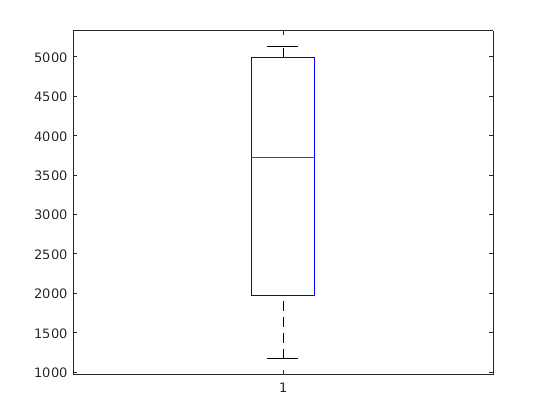
\includegraphics{Graphik/income1}
\begin{enumerate}
	\item Die Figur (..) zeigt das Boxplot-Diagramm von income1 
	\begin{itemize}
		\item Daten für ein Diagram müssen in einer Spalte liegen
		\item Daten müssen nicht sortiert sein
		\item Min- und Max-Werte sind jeweils durch den oberen bzw unteren Querstrich dargestllt
		\item Der Durschnitt (mean) ist der mittlere Abstand der äußeren  Striche
		\item Der Median (also das 50.Perzentil) wird durch den roten Querstricht innerhalb der Box dargestellt
		\item Q1 und Q3 sind jeweils Anfang bzw Ende der blauen Box
		\item um ein Boxplot-Diagram zu erstellen folgt man folgenden Schritten:
		\begin{enumerate}
			\item figure(1)
			\item boxplot(income1)
		\end{enumerate}
	\end{itemize}
	\item Die Figur (..) zeigt den Vergleich von income1 und income2
	\begin{itemize}
		\item Da sich die Anzahl der Datensätze verändert hat ist die Box (leicht) verschoben (also Q1 und Q3)
		\item aus den gleichen Gründen hat sich auch der Median verschoben 
		\item das rote Kreuz ist ein Ausreißer der sehr weit von dem Rest abweicht
	\end{itemize}
	\item Um vor Ausreißern gefeit zu sein empfiehlt sich die Betrachtung des Medians bei dichten Wertemengen
\end{enumerate}

\section*{4}
\begin{enumerate}
	\item Die folgenden Punkte beziehen sich auf das Kreisdiagram mit den Wahlergebnissen
	\begin{itemize}
		\item Beschriftung ist irreführend, da die Summe der angebenen  Verteilung > 100 \%
	\end{itemize}
	\item Die folgenden Punkte beziehen sich auf das Balkendiagram mit den Pokalen
	\begin{itemize}
		\item Die als 'Balken' gewählten Pokale sind schlecht zu vergleichen
		\item Es wird lediglich die Anzahl der gewonnen, nicht aber der gespielten Spiele angegeben
		\item Mangelde Details zum Verlauf der Spiele
	\end{itemize}
	\item Die folgenden Punkte beziehen sich auf die verbleibenden Diagramme
	\begin{itemize}
		\item Die vermeindlich zusammenpassenden Kurven liegen in verschiedenen Zeiten
	\end{itemize}
\end{enumerate}
		

\section*{5}
\begin{enumerate}
	\item 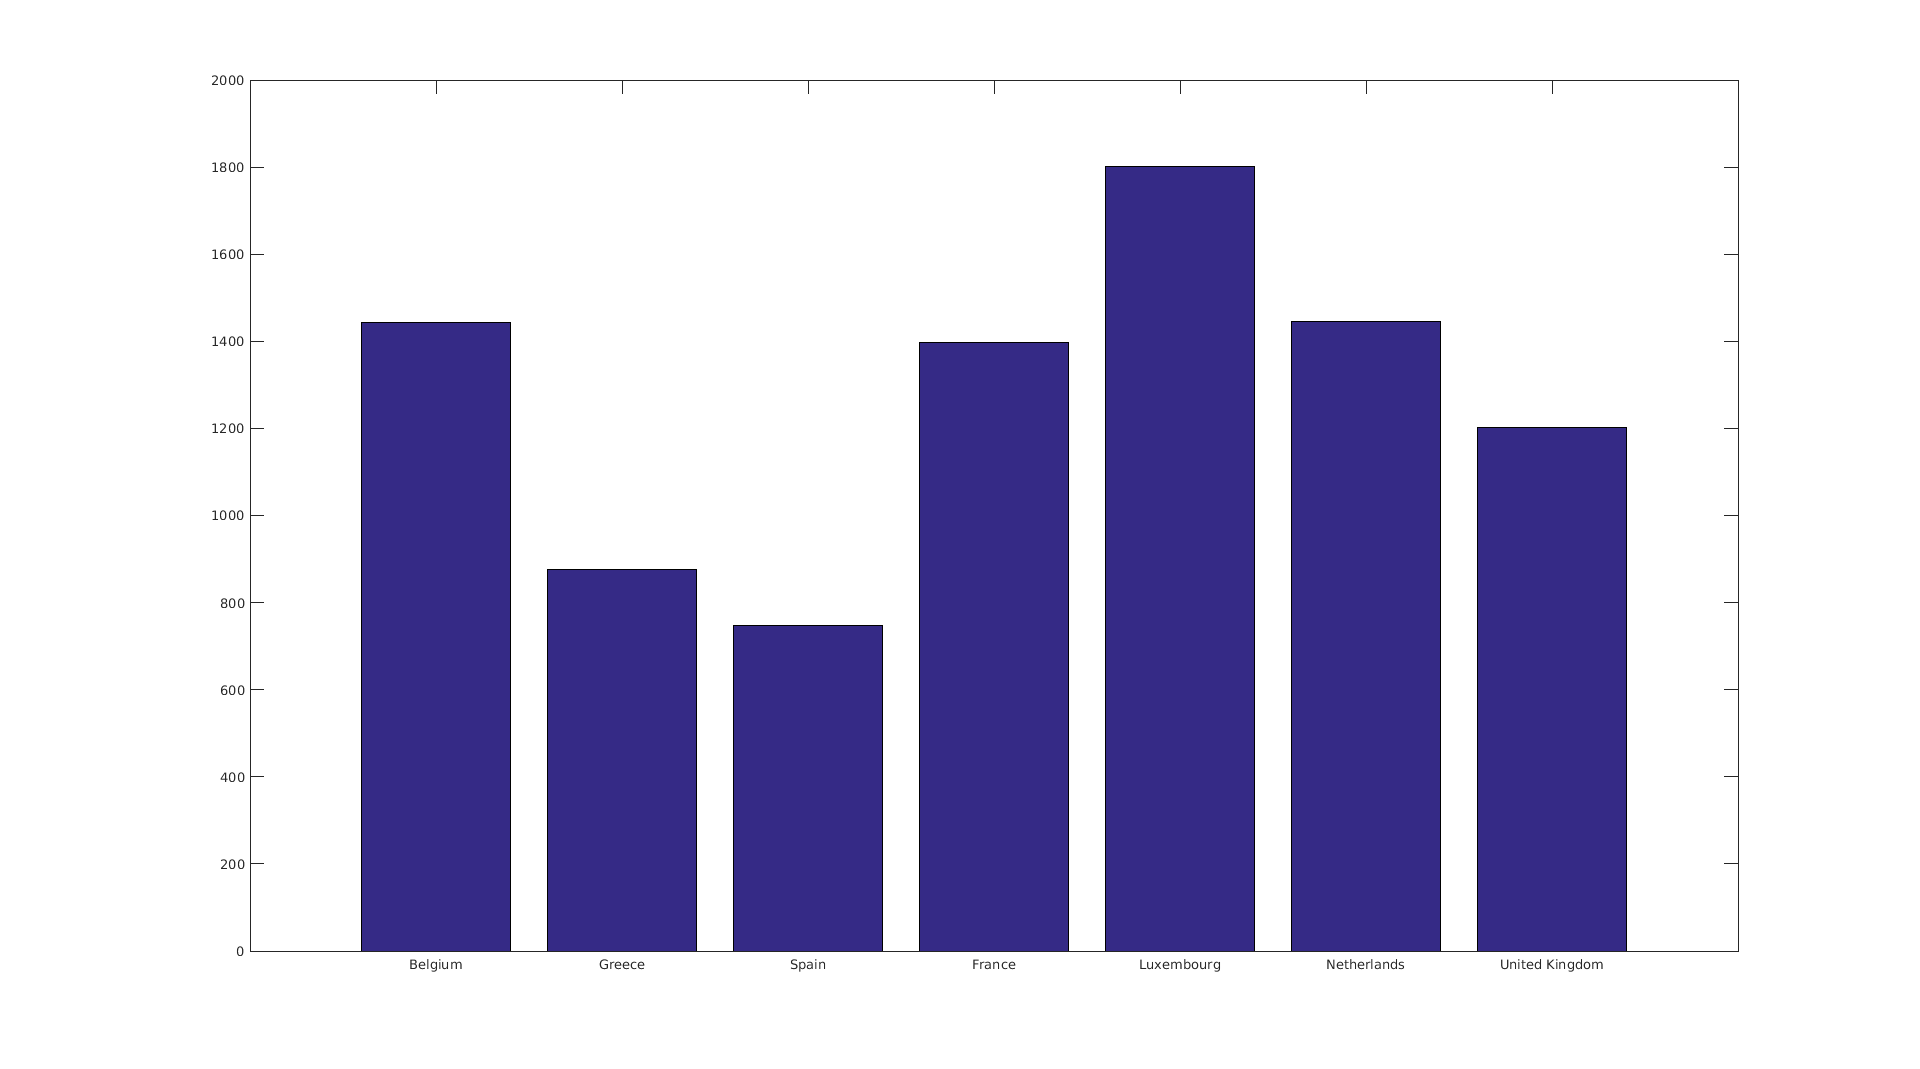
\includegraphics{Graphik/salary_bar}
	\item die Mindestlöhne illustrieren wir mithilfe eines Bar-Charts. Dafür sprechen folgende Punkte:
	\begin{itemize}
		\item es werden nur wenige verglichen
		\item die Werte sind ähnlich
		\item es besteht ein Interesse an dem direkten Vergleich der Werte
	\end{itemize}
	\item 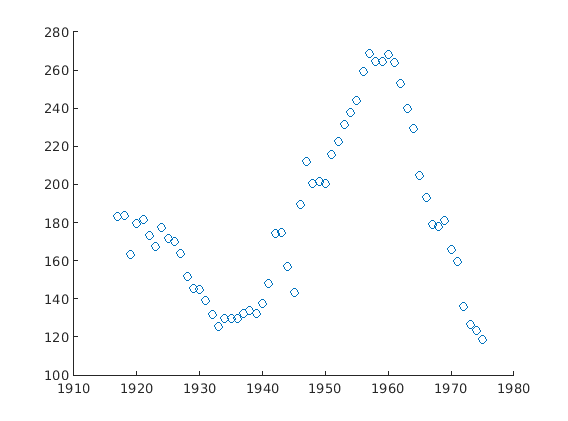
\includegraphics{Graphik/birthrates_scatter.png}
	\item die Geburtsrate stellen wir als Scatter-Plot da. Dafür sprechen folgende Punkte:
	\begin{itemize}
		\item die Daten sind als Tupel mit Zeitpunkt verfügbar
		\item es besteht ein Interesse an der Entwicklung
		\item die Datensätze sind standatisiert
	\end{itemize}
	\item 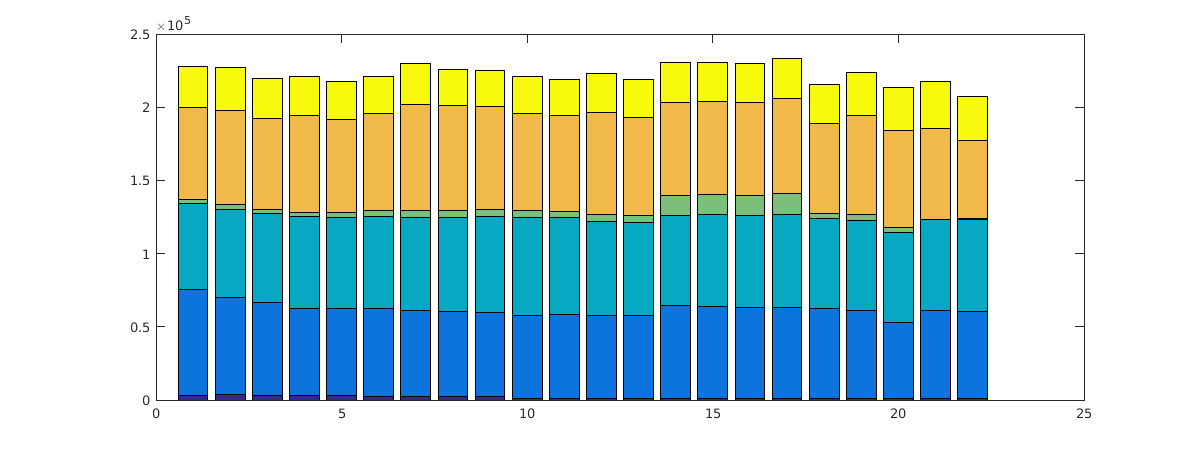
\includegraphics{Graphik/energy_bar}
	\item Die Energieverbrauchsstatistik geben wir als Bar-Chart an
	\begin{itemize}
		\item die 6 Spalten einer Zeile werden immer für eine Balken benutzt und farbig getrennt
		\item jeder Balken (jede Datenzeile) steht für ein Jahr
		\item dadurch lässt sich die Verteilung mehrer Jahre gut vergleichen
	\end{itemize}
	\item 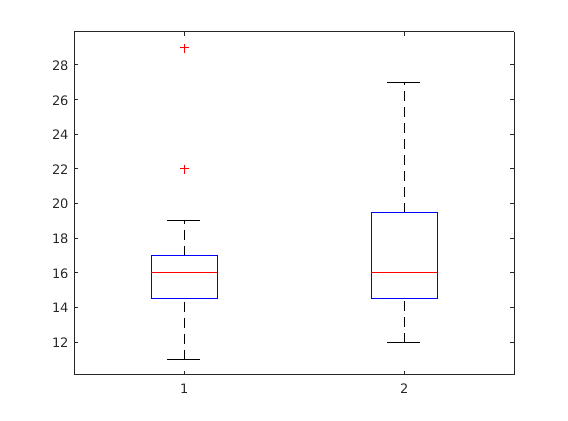
\includegraphics{Graphik/stroop_box}
	\item Für die Visualizierung des Stroop nehmen Boxplots
	\begin{itemize}
		\item zwei Datenreihen, die miteinander verglichen werden
		\item gleiches Experiment
		\item mehrere Ergebnisse
	\end{itemize}
	\item Das Klima wird als timeseries dargestellt
	\item 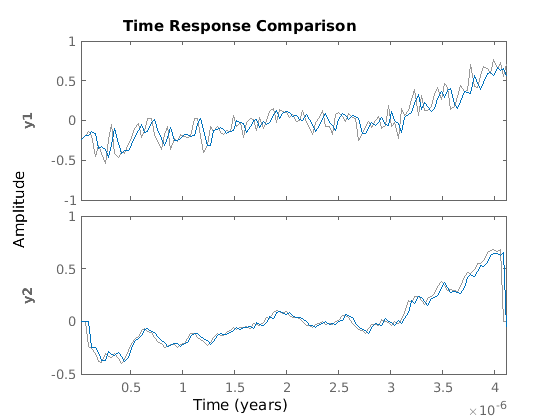
\includegraphics{Graphik/climate_timeseries}
\end{enumerate}

\end{document}

